\documentclass[conference,harvard,brazil,english]{sbatex}
\usepackage[latin1]{inputenc}
\usepackage{ae}
\usepackage{float}
\usepackage{graphicx}
\usepackage{caption}
\usepackage{subcaption}

\makeatletter
\def\verbatim@font{\normalfont\ttfamily\footnotesize}
\makeatother
\usepackage{amsmath}

% --------------------------------------------------
% --------------------------------------------------
% --------------------------------------------------


\begin{document}

% CABE?ALHO

\title{QUANTILE HASHING : A NAIVE LOCALITY SENSITIVE HASHING FOR A FAST APPROXIMATE NEAREST NEIGHBOURS CLASSIFICATION}

\author{Paulo Cirino Ribeiro Neto}{paulo-cirino@ufmg.br}
\address{Universidade Federal de Minas Gerais \\ Belo Horizonte, Minas Gerais, Brasil}

\twocolumn[

\maketitle

\selectlanguage{english}
\begin{abstract}

\end{abstract}

\keywords{Machine Learning, Classification,  Nearest Neighbor,  Locality Sensitive Hashing}

\selectlanguage{brazil}
\begin{abstract}
  Os artigos a serem submetidos dever?o ser redigidos em l?ngua portuguesa, espanhola ou inglesa, com n?mero m?ximo de 6 (seis) p?ginas, tamanho A4, coluna dupla, em formato PDF.
\end{abstract}

\keywords{Aprendizagem de m?quinas, Classifica??o, Reconhecimento de Padr?es, Hashing}
]

% CONTRIBUI??O

\selectlanguage{brazil}


% --------------------------------------------------
% --------------------------------------------------
% --------------------------------------------------

%%%%%%%%%%%%%%%%%%%%%%%%%%%%%%%%%%%%%%%%%%%%%%%%%%%%%%%%%%%%%%%%
%%%%%%%%%%%%%%%%%%%%%%%%%%%%%%%%%%%%%%%%%%%%%%%%%%%%%%%%%%%%%%%%
%%%%%%%%%%%%%%%%%%%%%%%%%%%%%%%%%%%%%%%%%%%%%%%%%%%%%%%%%%%%%%%%
\section{Introdu��o}



%%%%%%%%%%%%%%%%%%%%%%%%%%%%%%%%%%%%%%%%%%%%%%%%%%%%%%%%%%%%%%%%
%%%%%%%%%%%%%%%%%%%%%%%%%%%%%%%%%%%%%%%%%%%%%%%%%%%%%%%%%%%%%%%%
%%%%%%%%%%%%%%%%%%%%%%%%%%%%%%%%%%%%%%%%%%%%%%%%%%%%%%%%%%%%%%%%
\section{Metodologia}
\subsection{Formula��o}
\begin{figure}[H]
	\centering
	\begin{subfigure}[b]{0.225\textwidth}
		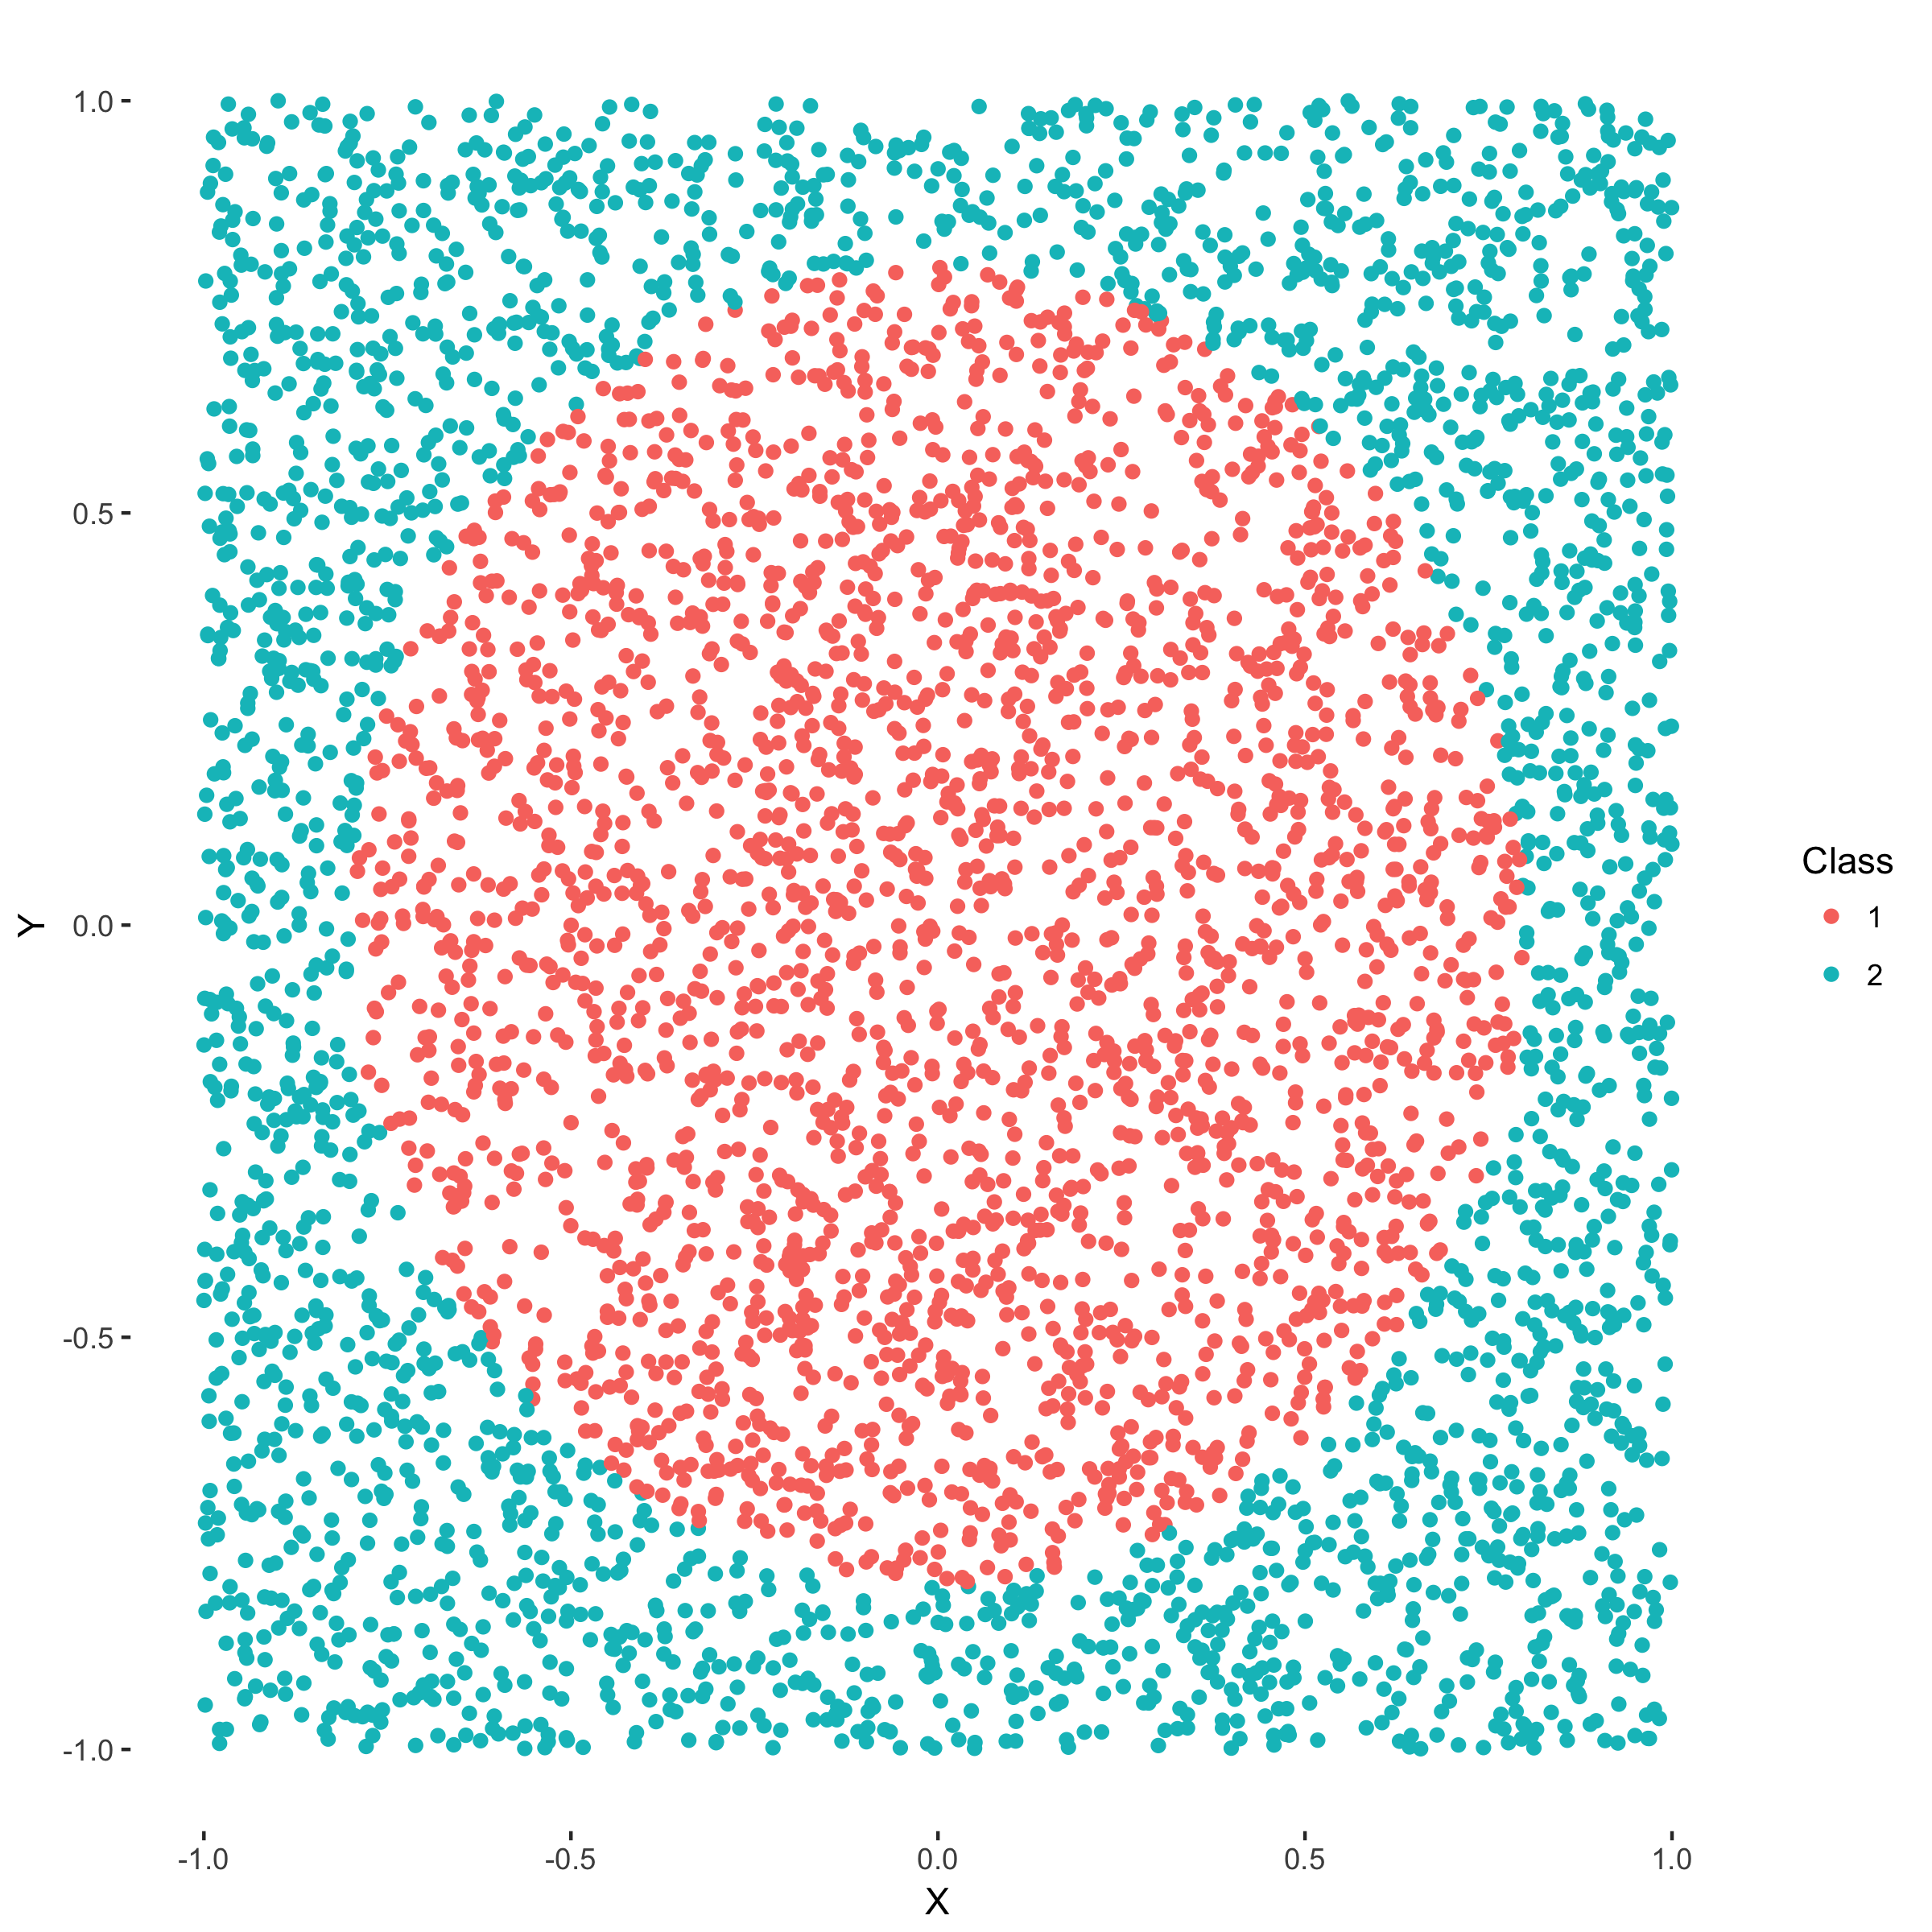
\includegraphics[width=\textwidth]{pics/data.png}
		\caption{Original Data Set}
		\label{fig:originalData}
	\end{subfigure}
	\begin{subfigure}[b]{0.225\textwidth}
		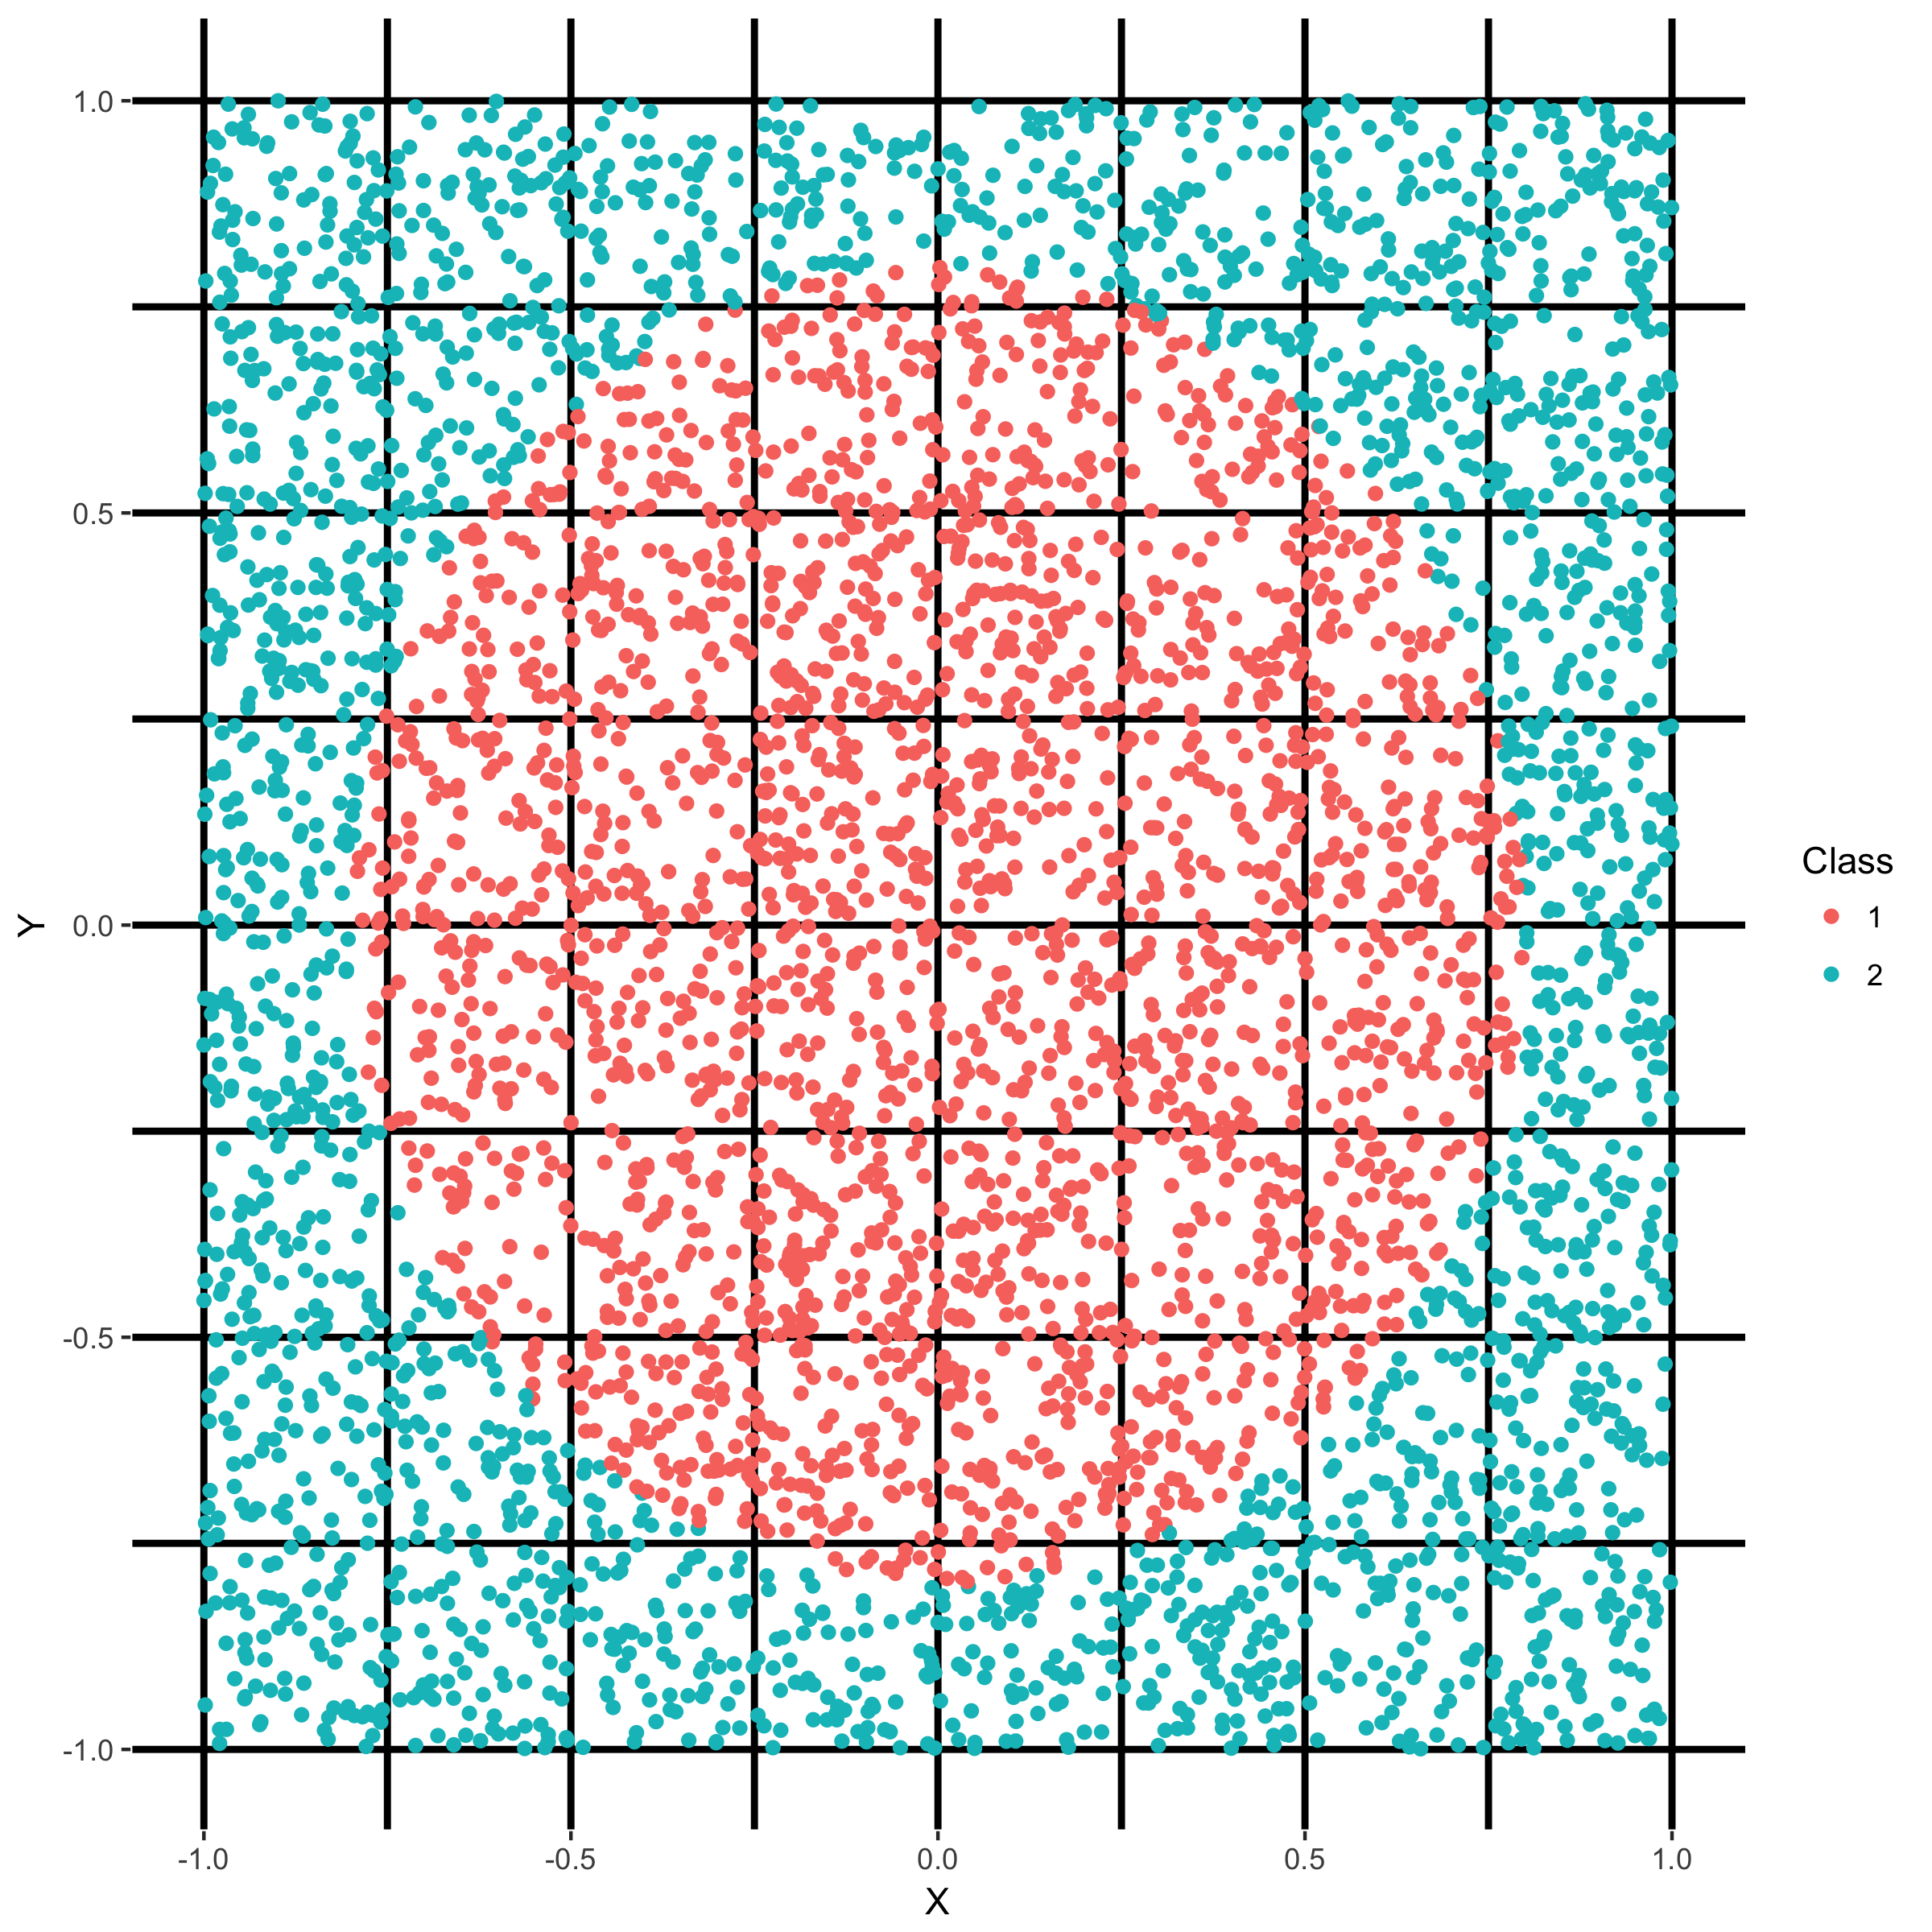
\includegraphics[width=\textwidth]{pics/grid.png}
		\caption{Grid on Data Set}
		\label{fig:gridData}
	\end{subfigure}
\end{figure}


\begin{figure}[H]
	\centering
	\begin{subfigure}[b]{0.225\textwidth}
		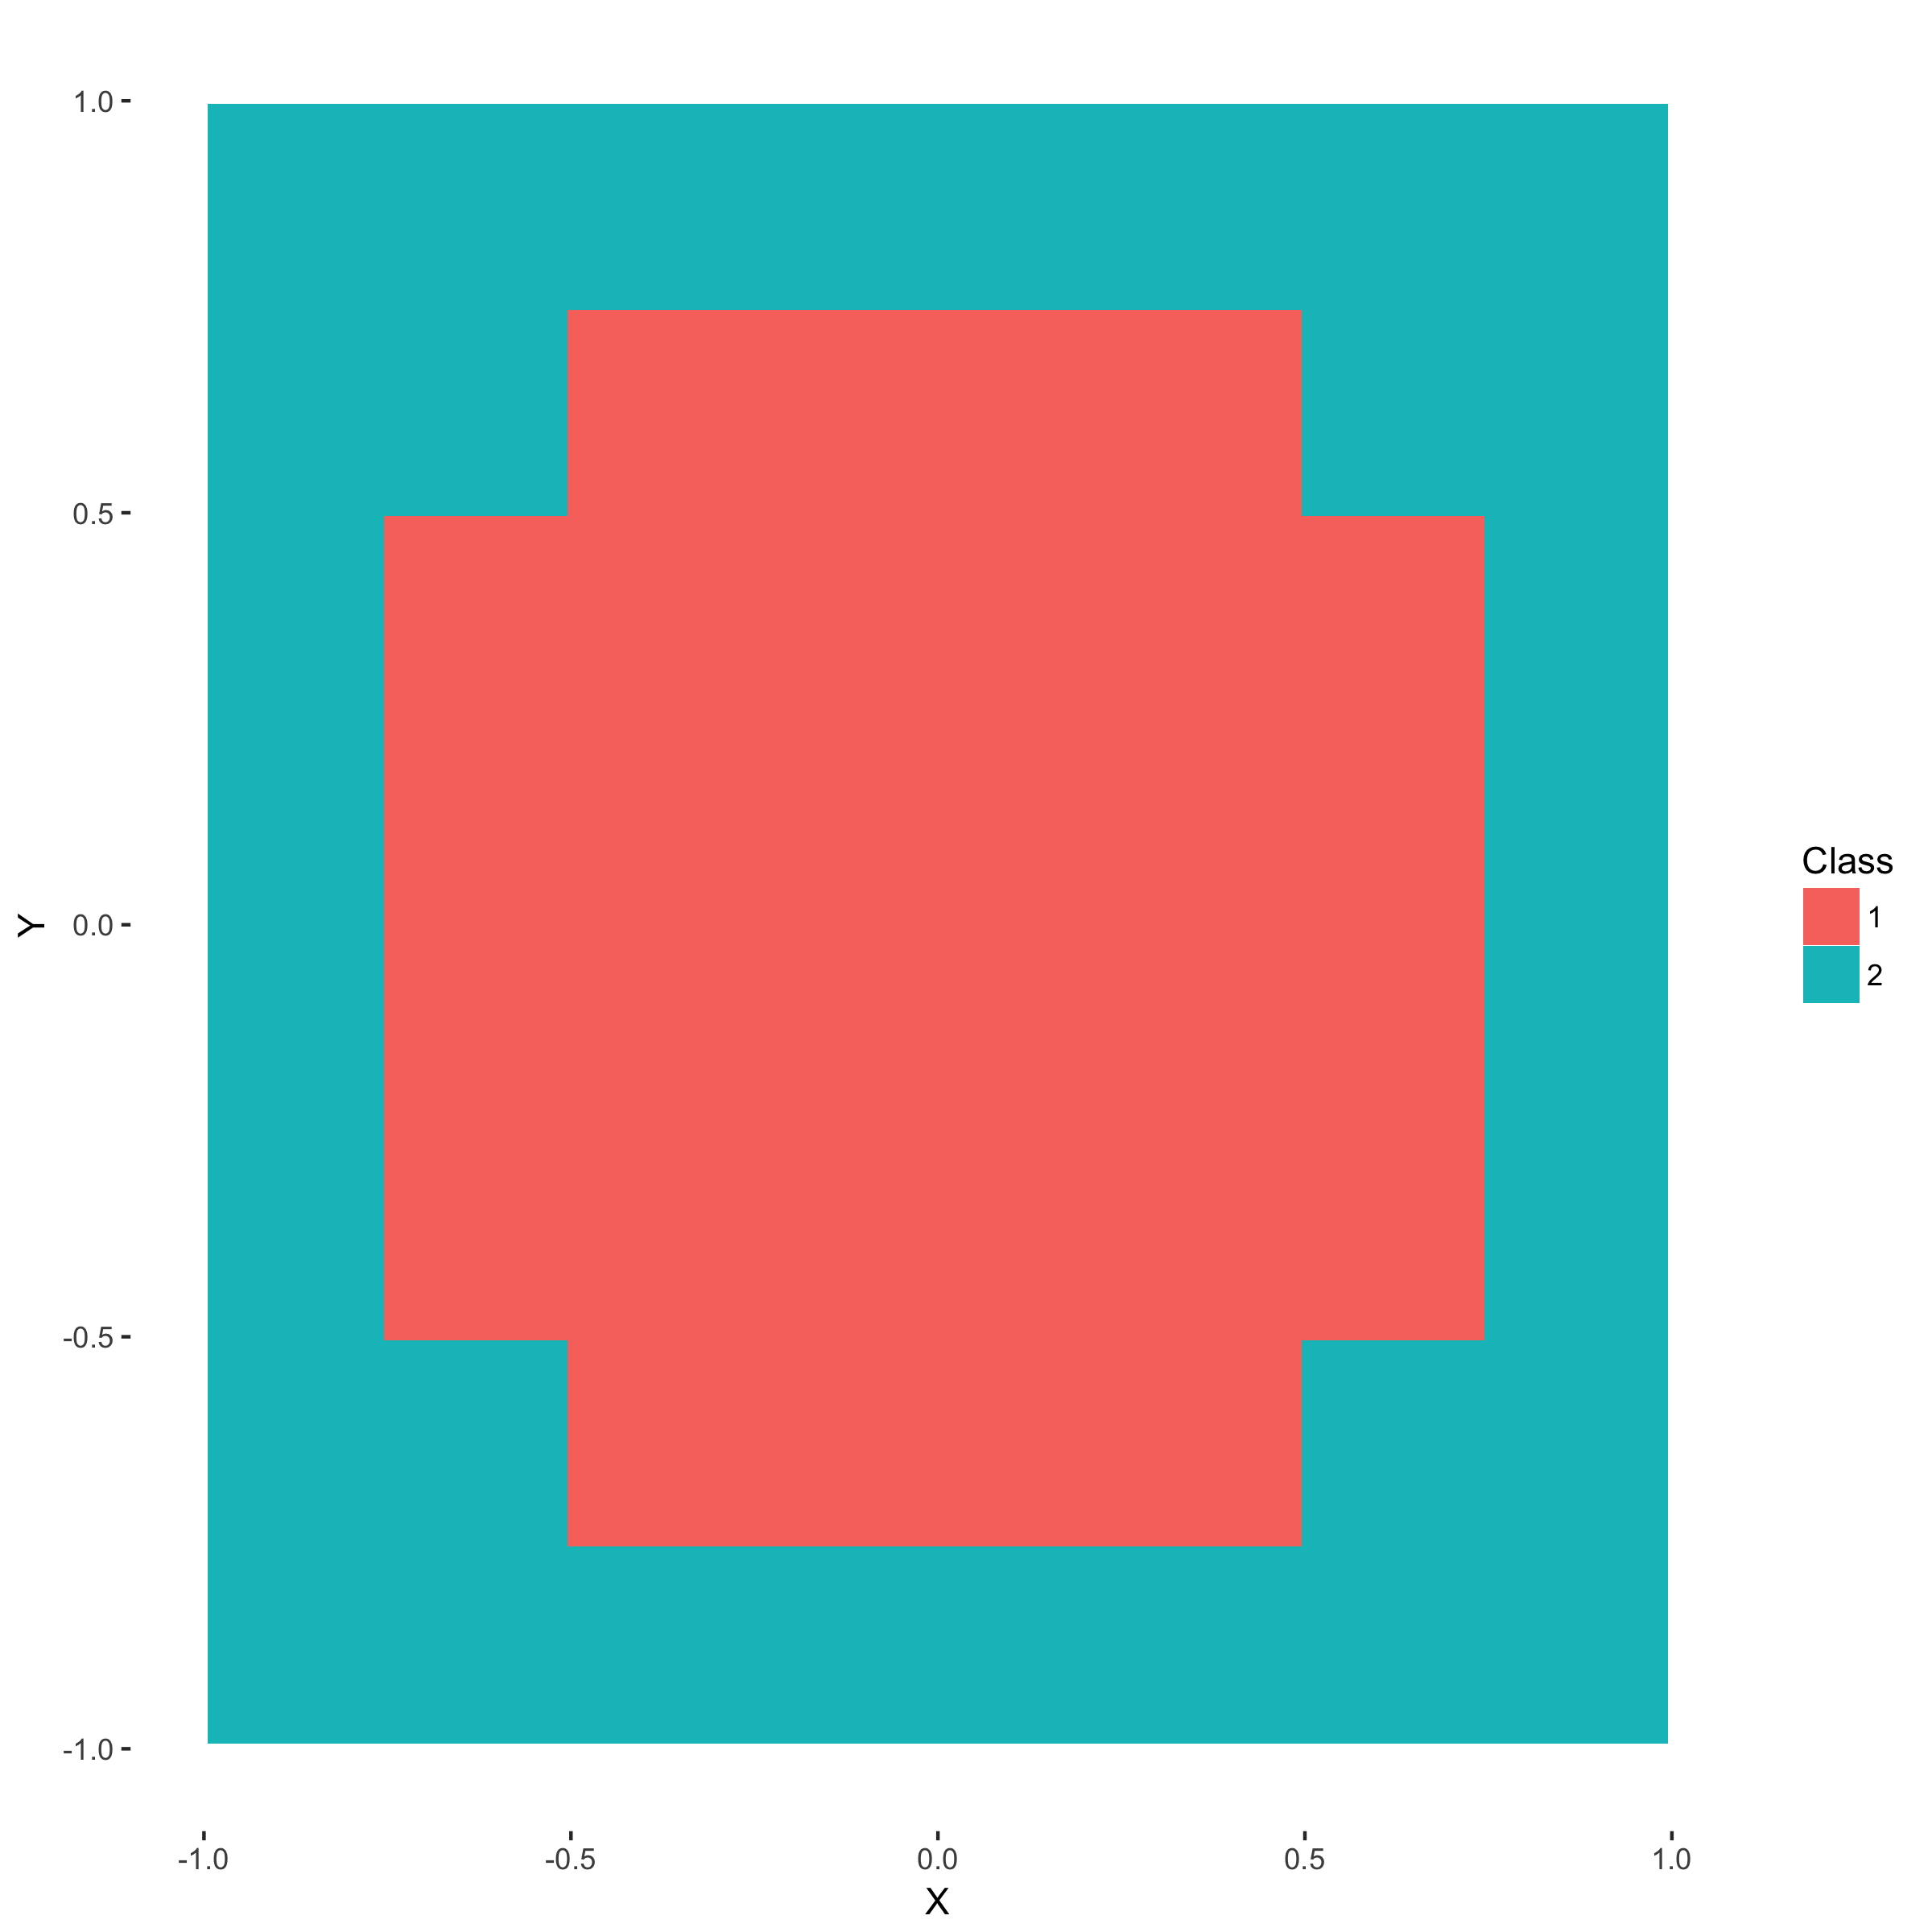
\includegraphics[width=\textwidth]{pics/dataClass3.png}
		\caption{Original Data Set}
		\label{fig:originalData}
	\end{subfigure}
	\begin{subfigure}[b]{0.225\textwidth}
		\includegraphics[width=\textwidth]{pics/dataClass5.png}
		\caption{Grid on Data Set}
		\label{fig:gridData}
	\end{subfigure}
\end{figure}


%%%%%%%%%%%%%%%%%%%%%%%%%%%%%%%%%%%%%%%%%%%%%%%%%%%%%%%%%%%%%%%%
%%%%%%%%%%%%%%%%%%%%%%%%%%%%%%%%%%%%%%%%%%%%%%%%%%%%%%%%%%%%%%%%
%%%%%%%%%%%%%%%%%%%%%%%%%%%%%%%%%%%%%%%%%%%%%%%%%%%%%%%%%%%%%%%%
\section{Experimentos}
\subsection{Defini��o do Experimento}
\subsection{Resultados}
\begin{table}[H]
	\centering
	\begin{tabular}{rrrrr}
		\hline
		& Cassini & Circle & Normals2D & XOR \\ 
		\hline
		KNN-1 & 100.00 & 99.54 & 88.35 & 99.67 \\ 
		KNN-3 & 100.00 & 99.52 & 90.46 & 99.67 \\ 
		KNN-5 & 100.00 & 99.51 & 91.06 & 99.66 \\ 
		KNN-7 & 100.00 & 99.52 & 91.34 & 99.66 \\ 
		QH-2 & 91.83 & 75.30 & 86.97 & 100.00 \\ 
		QH-3 & 97.89 & 94.93 & 90.58 & 100.00 \\ 
		QH-4 & 99.99 & 95.96 & 91.77 & 100.00 \\ 
		QH-5 & 100.00 & 97.76 & 91.87 & 100.00 \\ 
		QH-6 & 100.00 & 98.91 & 91.73 & 100.00 \\ 
		\hline
	\end{tabular}
\end{table}

%%%%%%%%%%%%%%%%%%%%%%%%%%%%%%%%%%%%%%%%%%%%%%%%%%%%%%%%%%%%%%%%
%%%%%%%%%%%%%%%%%%%%%%%%%%%%%%%%%%%%%%%%%%%%%%%%%%%%%%%%%%%%%%%%
%%%%%%%%%%%%%%%%%%%%%%%%%%%%%%%%%%%%%%%%%%%%%%%%%%%%%%%%%%%%%%%%
\section{Conclus�es}

\section{Trabalhos Futuros}

%%%%%%%%%%%%%%%%%%%%%%%%%%%%%%%%%%%%%%%%%%%%%%%%%%%%%%%%%%%%%%%%
%%%%%%%%%%%%%%%%%%%%%%%%%%%%%%%%%%%%%%%%%%%%%%%%%%%%%%%%%%%%%%%%
%%%%%%%%%%%%%%%%%%%%%%%%%%%%%%%%%%%%%%%%%%%%%%%%%%%%%%%%%%%%%%%%

\section*{Agradecimentos}


% --------------------------------------------------
% --------------------------------------------------
% --------------------------------------------------
% BIBLIOGRAFIA
\bibliography{exemplo}
\end{document}
